\documentclass[8pt,t,usepdftitle=false]{beamer}
\usetheme{Juelich}
\usepackage{setspace}
\usepackage[official]{eurosym}
\usepackage{bm}
\usepackage{mathtools}
%\usepackage{enumitem}\setitemize{itemsep=1ex}
\usepackage[%
backend=bibtex,
style=authoryear,
doi=true,
isbn=true,
url=true,
eprint=false,
sorting=nyt]{biblatex}
\addbibresource{refs.bib}
\usepackage{listings}
\lstset{
    basicstyle=\footnotesize,
    commentstyle=\color{blue},
    stringstyle=\sffamily,
    texcl=false,
    numbers=left,
    numberstyle=\tiny,
    stepnumber=1,
    numbersep=2ex,
    showstringspaces=false,
    captionpos=b,
    lineskip=0ex,%1pt,
    aboveskip=10pt,
    belowskip=10pt,
    frame=tb,
    showlines=true
}

\fzjset{
  title=regular,
  subtitle=regular,
  part=regular,
}

\setbeamerfont{title}{size*={10pt}{10pt},series=\bfseries}
\setbeamerfont{subtitle}{size*={12pt}{12pt},series=\bfseries\color{white}}
\setbeamerfont{frametitle}{size*={14pt}{14pt},series=\bfseries}
\setbeamertemplate{navigation symbols}{}

\setbeamertemplate{itemize/enumerate body begin}{\normalsize}
\setbeamertemplate{itemize/enumerate subbody begin}{\normalsize}
\setbeamertemplate{itemize/enumerate subsubbody begin}{\normalsize}
\setbeamertemplate{itemize/enumerate subsubsubbody begin}{\normalsize}

\mode<presentation>
{
  \usetheme{default}
  %% \setbeamercovered{transparent}
  \usefonttheme{professionalfonts}
  \usefonttheme{structurebold}
  \usecolortheme[rgb={0,0.3,0.6}]{structure}
}

% Delete this, if you do not want the table of contents to pop up at
% the beginning of each subsection:
% \AtBeginSection[]
% {
%   %\begin{frame}<beamer>
%     \begin{frame}[plain]
%     \frametitle{Outline}
%     \tableofcontents[currentsection]
%   \end{frame}
% }

\setlength{\leftmarginii}{3ex}

\setbeamercolor{alerted text}{fg=fzjblue}

\renewcommand{\arraystretch}{1.5}

\hypersetup{colorlinks,linkcolor=fzjblue,urlcolor=fzjblue,citecolor=fzjblue}

\newcommand{\Ex}{\text{E}}
\newcommand{\In}{\text{I}}
\newcommand{\inp}{\text{inp}}
\newcommand{\rest}{\text{rest}}
\newcommand{\tauM}{\tau_{\text{m}}}
\newcommand{\tauR}{\tau_{\text{ref}}{}}
\newcommand{\tauS}{\tau_{\text{S}}{}}

%%%%%%%%%%%%%%%%%%%%%%%%%%%%%%%%%%%%%%%%%%%%%%%%%%%%%%%%%%%%%%%%%%%%%%%%%%%%%%%%%%%%%%%%%%%%%%%%%
%% macros
\def\figpath{./figures}

\hypersetup{
  pdftitle={Introduction to NEST},
  pdfauthor={Tom Tetzlaff}
  }

%%%%%%%%%%%%%%%%%%%%%%%%%%%%%%%%%%%%%%%%%%%%%%%%%%%%%%%%%%%%%%%%%%%%%%%%%%%%%%%%%%
\title{%
  {\LARGE\bf Introduction to NEST}
  \hfill
\includegraphics[width=0.15\linewidth]{./figures/nest-logo}\\[1ex]
}
\subtitle{%
  {\normalsize\mdseries Tom Tetzlaff}%
  %{\hfill\tiny\url{t.tetzlaff{at}fz-juelich.de}}\\
  {\hfill\tiny\texttt{t.tetzlaff@fz-juelich.de}}\\  
  {\footnotesize\mdseries Institute of Neuroscience and Medicine (INM-6), J\"ulich Research Centre and JARA}
  %{\hfill\tiny\url{http://www.csn.fz-juelich.de}}
  {\hfill\tiny\texttt{http://www.csn.fz-juelich.de}}
  \\
  {\tiny\mdseries EITN fall school, Paris, 22.09.2023}
}
\date{}
\author{}
\institute{}

%%%%%%%%%%%%%%%%%%%%%%%%%%%%%%%%%%%%%%%%%%%%%%%%%%%%%%%%%%%%%%%%%%%%%%%%%%%%%%%%%%%%%%%%%%%%%%%%%
\begin{document}
\maketitle

%%%%%%%%%%%%%%%%%%%%%%%%%%%%%%%%%%%%%%%%%%%%%%%%%%%%%%%%%%%%%%%%%%%%%%%%%%%%%%%%%%%%%%%%%%%%%%%%%
\begin{frame}[plain]
  \begin{center}
    \parbox{0.9\linewidth}{
      \vspace{0.95\textheight}
      \parbox[c]{0.1\linewidth}{%
        \href{https://creativecommons.org/licenses/by-sa/4.0}{%
          
\includegraphics[width=\linewidth]{\figpath/by-sa.png}}}
      \parbox[c]{0.9\linewidth}{\scriptsize%
        ~~{}This presentation is provided under the terms of the Creative Commons Attribution-ShareAlike License 4.0.
      }
    }    
  \end{center}
\end{frame}
%%%%%%%%%%%%%%%%%%%%%%%%%%%%%%%%%%%%%%%%%%%%%%%%%%%%%%%%%%%%%%%%%%%%%%%%%%%%%%%%%%%%%%%%%%%%%%%%%
\def\ttl{Outline}
\pdfbookmark[2]{Outline}{Outline}
\begin{frame}[plain]
  \frametitle{\ttl}
  \tableofcontents
\end{frame}
%%%%%%%%%%%%%%%%%%%%%%%%%%%%%%%%%%%%%%%%%%%%%%%%%%%%%%%%%%%%%%%%%%%%%%%%%%%%%%%%%%%%%%%%%%%%%%%%%
\def\ttl{Overview and general features}\section{\ttl}
\begin{frame}[t,plain]
  \frametitle{\ttl}
  \begin{columns}
    \begin{column}{0.7\linewidth}
      \begin{itemize}\itemsep2ex
      \item<1-> \emph{NEST} = \emph{NE}ural \emph{S}imulation \emph{T}echnology
      \item<1-> main focus:
        \begin{itemize}
        \item[] structure and dynamics of large networks\\ of \emph{spiking point neurons}
        \end{itemize}
      \item<2-> contra indications: 
        \begin{itemize}
        \item[] neuron models with detailed neuronal morphology\\
          (see \emph{NEURON})
        \end{itemize}
      \item<3-> runs on laptops as well as supercomputers {\tiny\parencite{Helias12_26,Jordan18_2}}
      \item<3-> supported platforms:
        \begin{itemize}
        \item Linux
        \item Mac OS X
        \item Windows via virtual machine
        \end{itemize}
      \item<4-> sources:
        \begin{itemize}
        \item web: \url{https://www.nest-simulator.org}
        \item code: \url{https://github.com/nest/nest-simulator}
        \item docs: \url{https://nest-simulator.readthedocs.io}
        \end{itemize}
      \end{itemize}      
    \end{column}
    \begin{column}{0.3\linewidth}
      \vspace*{20ex}
      \onslide<3->{
        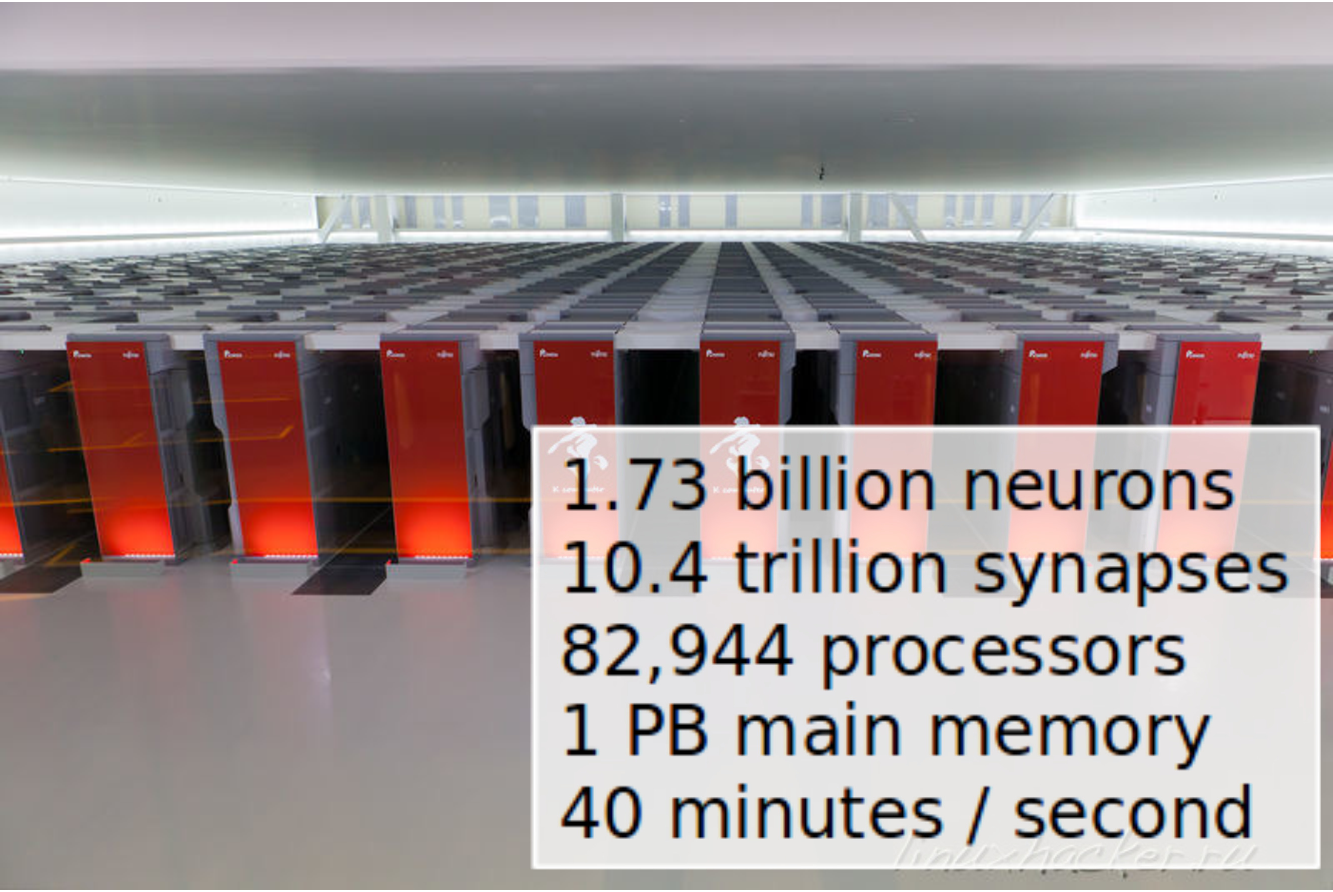
\includegraphics[width=\linewidth]{./figures/K.pdf}
      }
    \end{column}
  \end{columns}
\end{frame}
%%%%%%%%%%%%%%%%%%%%%%%%%%%%%%%%%%%%%%%%%%%%%%%%%%%%%%%%%%%%%%%%%%%%%%%%%%%%%%%%%%%%%%%%%%%%%%%%% 
%%%%%%%%%%%%%%%%%%%%%%%%%%%%%%%%%
\begin{frame}[t,plain]
  \frametitle{\ttl}
  \begin{itemize}\itemsep2ex
  \item<1-> open-source software, licensed under GNU General Public License
    \begin{itemize}
    \item first release: ``SYNOD'' (1994)
    \item latest release: NEST 3.5 (Feb.~2023)
    \end{itemize}
  \item<2-> C++ kernel
  \item<2-> Python frontend \emph{PyNEST}
  \item<3-> hybrid parallelization:
    \begin{itemize}
    \item multi-threading for efficient usage of multi-processor machines
    \item MPI-parallelism for computer clusters and super computers 
    \end{itemize}
  \item<4-> large user community {\tiny (see \url{https://www.nest-simulator.org/community})}
    \begin{itemize}
    \item active \href{https://www.nest-simulator.org/mailinglist/postorius/lists/users.nest-simulator.org/}{user mailing list} with short response latencies
    \item yearly NEST conference {\tiny (see \url{https://nest-simulator.org/conference})}
    \end{itemize}
  \item<5-> development
    \begin{itemize}
    \item driven by scientific needs
    \item focus on efficiency, flexibility, accuracy, and reproducibility
    \item based on agile, continuous-integration workflows
    \end{itemize}
  \item<6-> citing NEST: see
    \href{https://zenodo.org/search?page=1&size=20&q=title:NEST\%20AND\%20-description:graphical&file_type=gz&sort=-publication_date}{Zenodo}, e.g.~\parencite{Nest340}    
  \end{itemize}    
\end{frame}
%%%%%%%%%%%%%%%%%%%%%%%%%%%%%%%%%
\def\ttl{Built-in neuron models}\section{\ttl}
\begin{frame}[t,plain]
  \frametitle{\ttl}
  \begin{itemize}
  \item integrate-and-fire models (\texttt{iaf\_*}, \texttt{*if\_*}) 
    \begin{itemize}\itemsep1ex
    \item with current-based (\texttt{iaf\_psc\_*})
    \item and conducance based synapses (\texttt{iaf\_cond\_*})
    \item and different synaptic kernels (\texttt{*\_delta}, \texttt{*\_exp}, \texttt{*\_alpha})
    \end{itemize}
  \item adaptive exponential IaF models (AdEx; \texttt{aeif\_*})
  \item generalized leaky integrate-and-fire models (glif; \texttt{gif\_*})
  \item multi-timescale adaptive threshold model (\texttt{mat2\_*},\texttt{amat2\_*})
  \item Izhikevich model (\texttt{izhikevich})
  \item Hodgkin-Huxley type models (\texttt{hh\_*})
  \item neuron models with multiple (few) compartments (\texttt{*\_mc\_*})
  \item firing rate neurons (\texttt{tanh\_*}, \texttt{threshold\_lin\_*}, \texttt{sigmoid\_*}, \texttt{siegert\_*})
  \item binary neuron models (\texttt{mcculloch\_pitts\_*}, \texttt{ginzburg\_*})
  \item \ldots and many more
  \end{itemize}
  \hspace*{\fill}{\tiny (for an overview of all built-in models, see \url{https://nest-simulator.readthedocs.io/en/stable/models})}   
\end{frame}
%%%%%%%%%%%%%%%%%%%%%%%%%%%%%%%%%
\def\ttl{Built-in synapse models}\section{\ttl}
\begin{frame}[t,plain]
  \frametitle{\ttl}
  \begin{itemize}
  \item current-based and conductance-based synapses (see neuron models)
  \item \href{https://nest-simulator.readthedocs.io/en/stable/models/gap_junction.html}{gap junctions} (\texttt{gap\_junction}) 
  \item static synapses (\texttt{static\_synapse*})
  \item various types of synaptic plasticity
    \begin{itemize}\itemsep1ex
    \item various forms of short term plasticity (\texttt{tsodyks*}, \texttt{quantal\_stp\_*})
    \item various forms of spike-timing-dependent plasticity (\texttt{stdp\_*})
    \item STDP plus third factors (\texttt{clopath\_*}, \texttt{stdp\_dopamine\_*})
    \item \href{https://nest-simulator.readthedocs.io/en/stable/auto_examples/structural_plasticity.html}{structural plasticity} {\tiny\parencite{Butz13_e1003259}}
    \end{itemize}
  \item stochastic synapses (synaptic failure; \texttt{bernoulli\_synapse})
  \item \ldots and many more
\end{itemize}
\hspace*{\fill}{\tiny (for an overview of all built-in models, see \url{https://nest-simulator.readthedocs.io/en/stable/models})}   
\end{frame}
%%%%%%%%%%%%%%%%%%%%%%%%%%%%%%%%%
\def\ttl{Custom neuron and synapse models with NESTML}\section{\ttl}
\begin{frame}[t,plain]
  \frametitle{\ttl}
  \begin{itemize}
  \item domain-specific language for neuron and synapse models\\[3ex]    
    \begin{center}
      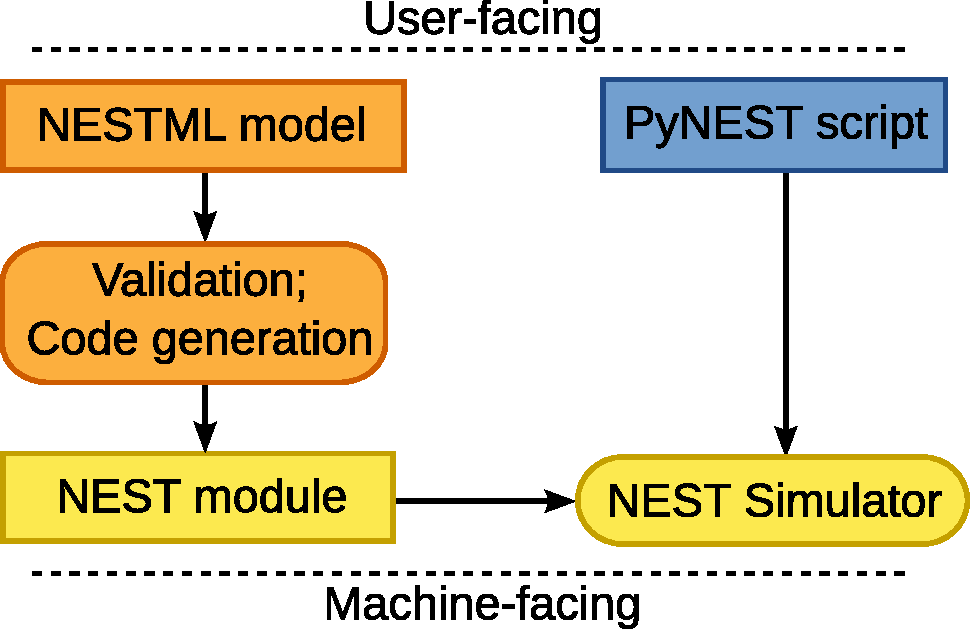
\includegraphics[width=0.7\linewidth]{./figures/nestml-workflow.pdf}
    \end{center}
    \vspace*{4ex}
  \item code: \url{https://github.com/nest/nestml}
  \item docs: \url{https://nestml.readthedocs.io}
  \item[] \vspace*{-5ex}\hfill
\includegraphics[width=0.2\linewidth]{./figures/nestml-logo.pdf}
  \end{itemize}
\end{frame}
%%%%%%%%%%%%%%%%%%%%%%%%%%%%%%%%%
\def\ttl{Stimulation devices}\section{\ttl}
\begin{frame}[t,plain]
  \frametitle{\ttl}
    \emph{Spike generators}
  \begin{itemize}
    \item spikes at prescribed points in time: \texttt{spike\_generator}
    \item realizations of homogeneous or inhomogeneous Poisson point processes:
      \begin{itemize}
      \item \texttt{poisson\_generator}
      \item \texttt{inhomogeneous\_poisson\_generator}
      \item \texttt{sinusoidal\_poisson\_generator}
      \end{itemize}
    \item realizations of homogeneous or inhomogeneous Gamma point processes:
      \begin{itemize}
      \item \texttt{gamma\_sup\_generator}\
      \item \texttt{sinusoidal\_gamma\_generator}
      \end{itemize}
  \end{itemize}
  \vspace*{2ex}
  \emph{Current generators}
  \begin{itemize}
    \item constant current: \texttt{dc\_generator}
    \item sinusoidal current: \texttt{ac\_generator}
    \item step-wise constant current: \texttt{step\_current\_generator}
    \item  noisy current: \texttt{noise\_generator}
    \end{itemize}
    \hspace*{\fill}{\tiny (see \url{https://nest-simulator.readthedocs.io/en/stable/devices/stimulate_the_network.html})}   
\end{frame}
%%%%%%%%%%%%%%%%%%%%%%%%%%%%%%%%%
\def\ttl{Recording devices}\section{\ttl}
\begin{frame}[t,plain]
  \frametitle{\ttl}
   \begin{itemize}
    \item spikes : \texttt{spike\_recorder} 
    \item analog quantities (membrane potentials, conductances, \ldots): \texttt{multimeter} 
    \item synaptic weights: \texttt{weight\_recorder}
    \end{itemize}
    \hspace*{\fill}{\tiny (see \url{https://nest-simulator.readthedocs.io/en/stable/devices/record_from_simulations.html})}
\end{frame}
%%%%%%%%%%%%%%%%%%%%%%%%%%%%%%%%%
\def\ttl{Connection management}\section{\ttl}
\begin{frame}[t,plain]
  \frametitle{\ttl}
  \begin{itemize}
  \item large repertoire of efficient built-in connection routines {\tiny\parencite{Ippen2017_30}}, incl.
    \begin{itemize}
    \item various forms of deterministic and random connectivity patterns
    \item spatially structured networks
    \end{itemize}
    {\tiny (see \url{https://nest-simulator.readthedocs.io/en/stable/synapses/connection_management.html})}  
  \end{itemize}
  \begin{center}
    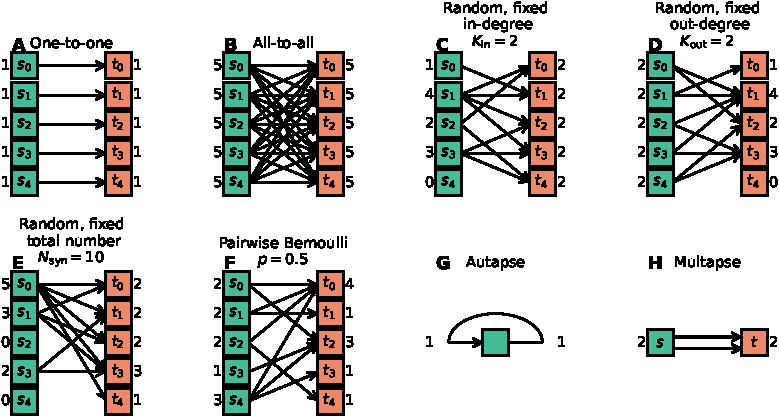
\includegraphics[width=0.9\linewidth]{./figures/SenkEtAl2022_connectivity_patterns_fig7.pdf}
  \end{center}
  \hspace*{\fill}{\tiny\parencite{Senk22_e1010086}}
\end{frame}
%%%%%%%%%%%%%%%%%%%%%%%%%%%%%%%%%
\def\ttl{Parametrization}\section{\ttl}
\begin{frame}[t,plain]
  \frametitle{\ttl}
  \begin{itemize}\itemsep2ex
  \item<1-> parameters: specification of, e.g.,
    \begin{itemize}\itemsep1ex
    \item initial conditions
    \item neuron or device properties
    \item positions in physical space
    \item connection probabilities, synaptic weights, delays
    \end{itemize}
  \item<2-> parameter types:
    \begin{itemize}\itemsep1ex
    \item random parameters (built-in RNGs)\\
      {\tiny (see \url{https://nest-simulator.readthedocs.io/en/stable/nest_behavior/random_numbers.html})}
    \item spatial parameters
    \item spatially distributed parameters
    \item mathematical functions
    \item clipping, redrawing, and conditional parameters
    \item combination of parameters
    \end{itemize}
  \end{itemize}
  \vfill\hspace*{\fill}{\tiny (see \url{https://nest-simulator.readthedocs.io/en/stable/neurons/parametrization.html})}
\end{frame}

%%%%%%%%%%%%%%%%%%%%%%%%%%%%%%%%%%%%%%%%%%%%%%%%%%%%%%%%%%%%%%%%%%%%%%%%%%%%%%%%%%%%%%%%%%%%%%%%%
\def\ttl{``Hello world!''}\section{\ttl}
\begin{frame}[t,plain]
  \frametitle{\ttl}
  \vspace*{-3ex}
  \onslide<1->{
    \lstinputlisting[firstnumber=auto,language=Python,name=helloworld,showstringspaces=false]
    {../code/pynest/hello_world.py}
    %% 
    \vspace*{-2ex}{\tiny (see \texttt{hello\_world.py})}\\
  }
  \onslide<2->{
    \vspace*{-3.8cm}
    \hspace*{\fill}
    \fcolorbox{black}{white}{\parbox{0.4\linewidth}{
        \footnotesize
        \texttt{hello\_world.pdf}:\\
        \includegraphics[width=\linewidth]{../code/pynest/figures/hello_world.pdf}
      }}
  }
\end{frame}
%%%%%%%%%%%%%%%%%%%%%%%%%%%%%%%%%%%%%%%%%%%%%%%%%%%%%%%%%%%%%%%%%%%%%%%%%%%%%%%%%%%%%%%%%%%%%%%%%
\def\ttl{Example: balanced random network}\section{\ttl}
%%%%%%%%%%%%%%%%%%%%%%%%%%%%%%%%%%%%%%%%%%%%%
\begin{frame}[t,plain]
  \frametitle{\ttl}
  \begin{columns}
    \column{0.5\linewidth}
    \centering
    \parbox{\linewidth}{\footnotesize
      \begin{itemize}
      \item[] simple model of a local cortex volume {\tiny\parencite{Brunel00_183}}\\
      ($\sim{}1\text{mm}^3$, $\sim{}10^{4\ldots{}5}$ neurons)
      \end{itemize}
    }\\
    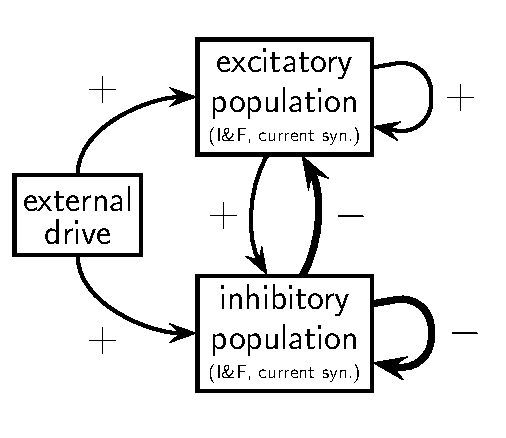
\includegraphics[width=0.8\linewidth]{figures/brunel}
    %%% 
    \column{0.5\linewidth}
    \centering
    \hspace{4ex}Connectivity matrix $J=\{J_{ij}\}$\\
    \rotatebox{90}{\hspace{12ex}post}
    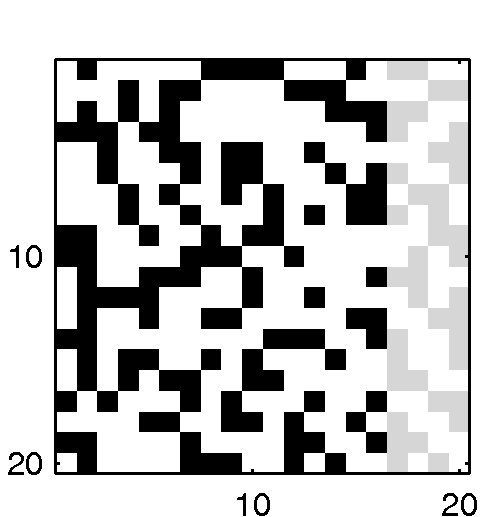
\includegraphics[width=0.6\linewidth]{figures/dalemat}\\
    \hspace{3ex}pre
  \end{columns}
  \begin{itemize}
  \item<1> $N_\Ex$ excitatory, $N_\In$ inhibitory neurons,
    $N=N_\Ex+N_\In\sim{}10^{4\ldots{}5}$
  \item<1> sparse, random connectivity with fixed in-degree $K=N/10$ 
  \item<1> LIF dynamics with current-based synapses with exponential shape:
    \begin{eqnarray*}
      \tauM{}\dot{V}_i &=& -V_i(t)+R\left(I_{i}^\text{net}(t)+I^\text{ext}\right)
                           \quad(i\in\{1,\ldots,N\})\\
      I_{i}^\text{net}(t) &=& \sum_{j} J_{ij} (h*s_j)(t-d)
                              \quad\text{with}\quad{}h(t)=e^{-t/\tauS}\Theta(t)
    \end{eqnarray*}
  \end{itemize}
\end{frame}
%%%%%%%%%%%%%%%%%%%%%%%%%%%%%%%%%%%%%%%%%%%%%
\begin{frame}[t,plain]
  \frametitle{\ttl}
  \begin{columns}
    \column{0.5\linewidth}
    \centering
    \parbox{\linewidth}{\footnotesize
      \begin{itemize}
      \item[] simple model of a local cortex volume {\tiny\parencite{Brunel00_183}}\\        
      ($\sim{}1\text{mm}^3$, $\sim{}10^{4\ldots{}5}$ neurons)
      \end{itemize}
    }\\
    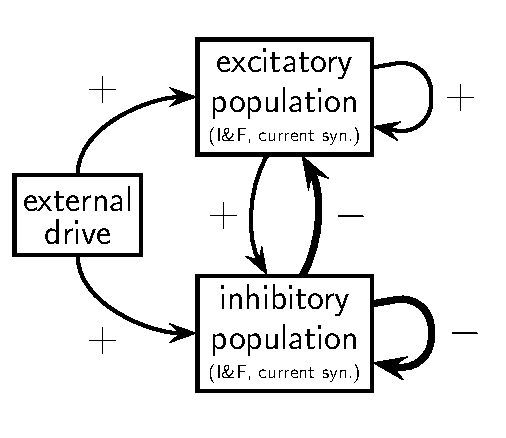
\includegraphics[width=0.8\linewidth]{figures/brunel}\\[-2ex]
    \begin{itemize}
    \item<1-> in-vivo like activity
      \begin{itemize}\normalsize
      \item large membrane potential fluctuations
      \item low firing rates
      \item irregular spiking
      \end{itemize}
    \item<1-> global oscillatory modes in various frequency
      bands
    \end{itemize}
    %%% 
    \column{0.5\linewidth}
    \footnotesize
    \centering
    \only<1->{
      \ \\[-0.5cm]
      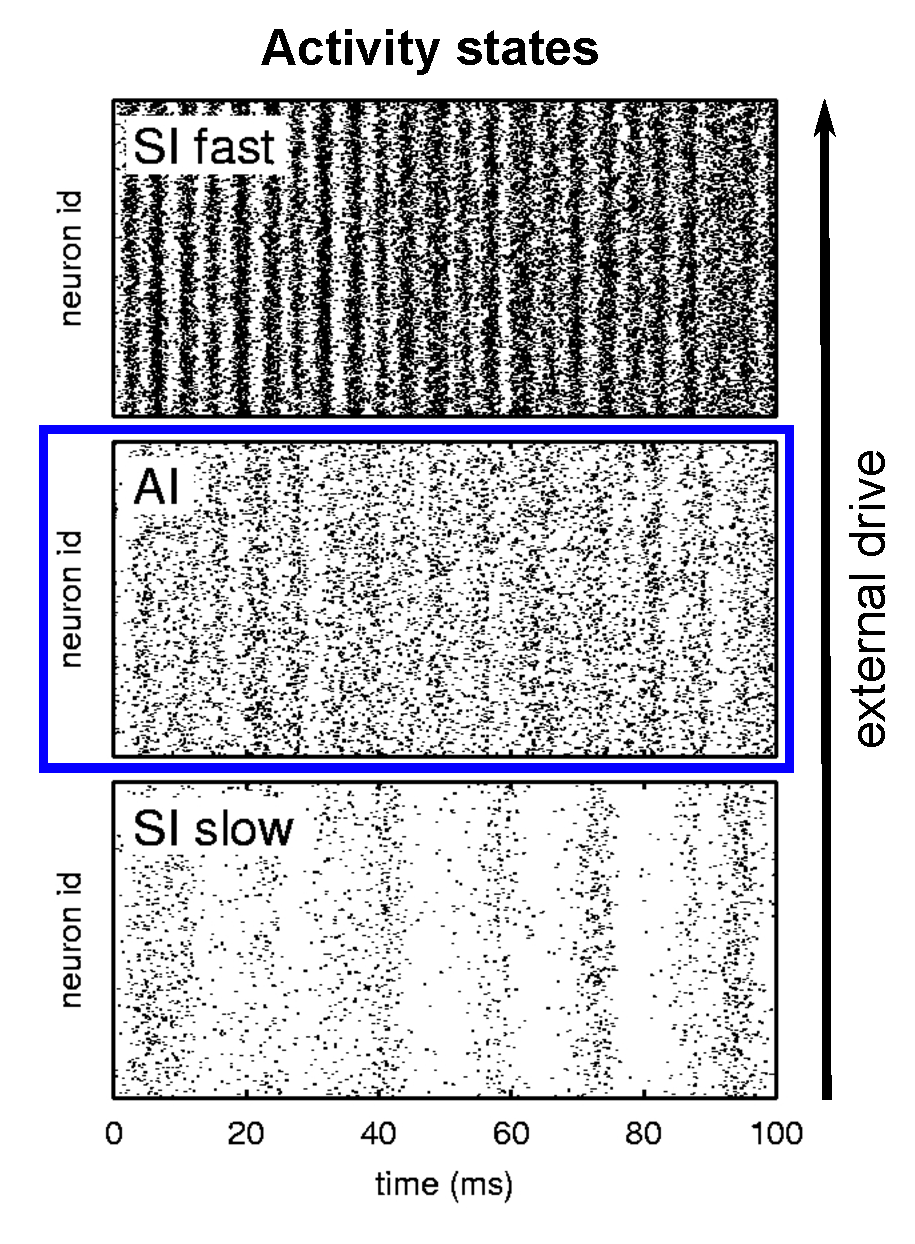
\includegraphics[width=\linewidth]{figures/brunel_all_states_mod.pdf}
    }
  \end{columns}
\end{frame}
%%%
\begin{frame}[t,plain]
  \frametitle{\ttl}
  implementation: see \texttt{balanced\_random\_network.py}
  \begin{center}
    \includegraphics[width=0.8\linewidth]{../code/pynest/figures/balanced_random_network.pdf}
  \end{center}
\end{frame}
%%%%%%%%%%%%%%%%%%%%%%%%%%%%%%%%%%%%%%%%%%%%%%%%%%%%%%%%%%%%%%%%%%%%%%%%%%%%%%%%%%%%%%%%%%%%%%%%%
\def\ttl{Acknowledgments}\section*{\ttl}
\begin{frame}[plain]
  \frametitle{\ttl}
  This presentation is based on previous work by many people, in particular:\\[3ex]
  \begin{columns}
    \begin{column}{0.5\linewidth}
      \begin{itemize}
        \item Hannah Bos
        \item David Dahmen
        \item Moritz Deger
        \item Jochen Martin Eppler
        \item Espen Hagen
        \item Charl Linssen          
      \end{itemize}
    \end{column}
    \begin{column}{0.5\linewidth}
      \begin{itemize}
        \item Abigail Morrison        
        \item Jannis Schuecker
        \item Johanna Senk
        \item Tom Tetzlaff
        \item Sacha van Albada
        \item Alexander van Meegen          
      \end{itemize}
    \end{column}
  \end{columns}
\end{frame}
%%%%%%%%%%%%%%%%%%%%%%%%%%%%%%%%%%%%%%%%%%%%%%%%%%%%%%%%%%%%%%%%%%%%%%%%%%%%%%%%%%%%%%%%%%%%%%%%%
\begin{frame}[t,plain,allowframebreaks]
  \begin{center}
    \vspace*{\fill}
    \LARGE\emph{\it Thanks}
    \vspace*{\fill}
  \end{center}
\end{frame}
%%%%%%%%%%%%%%%%%%%%%%%%%%%%%%%%%%%%%%%%%%%%%%%%%%%%%%%%%%%%%%%%%%%%%%%%%%%%%%%%%%%%%%%%%%%%%%%%%
%% references
\setbeamertemplate{bibliography item}{}  %% remove document icon
\def\ttl{References}\section*{\ttl}
\begin{frame}[t,plain,allowframebreaks]  
  \frametitle{\ttl}
  \bibitemsep1ex
  \renewcommand{\bibfont}{\normalfont\small}
  \printbibliography
\end{frame}
%%%%%%%%%%%%%%%%%%%%%%%%%%%%%%%%%%%%%%%%%%%%%%%%%%%%%%%%%%%%%%%%%%%%%%%%%%%%%%%%%%%%%%%%%%%%%%%%%
\end{document}
%%%%%%%%%%%%%%%%%%%%%%%%%%%%%%%%%%%%%%%%%%%%%%%%%%%%%%%%%%%%%%%%%%%%%%%%%%%%%%%%%%%%%%%%%%%%%%%%%
%%%%%%%%%%%%%%%%%%%%%%%%%%%%%%%%%%%%%%%%%%%%%%%%%%%%%%%%%%%%%%%%%%%%%%%%%%%%%%%%%%%%%%%%%%%%%%%%%

%%% Local Variables:
%%% mode: latex
%%% TeX-master: t
%%% End:
